\documentclass{ximera}

\title{This is the sample!}

\newcommand{\mypreamble}{WHEEEEE}
%%% Local Variables:
%%% mode: latex
%%% TeX-master: t
%%% End:


\begin{document}
\begin{abstract}
  The begining and now an instructor! I am doing math like $\arcsin$.
\end{abstract}

\maketitle

\mypreamble

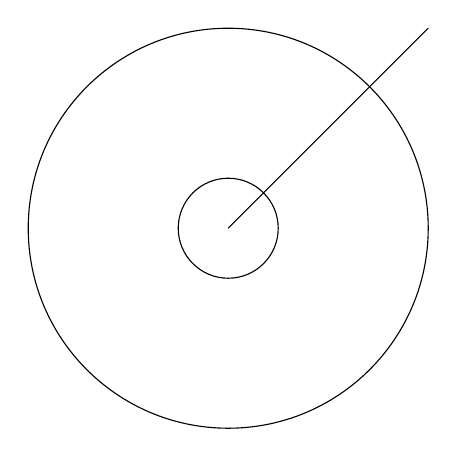
\begin{tikzpicture}
  \draw (0,0) circle (1in);
  \draw (0,0) circle (0.25in);
  \draw (0,0) -- (1in,1in);
\end{tikzpicture}

\youtube{eGXGlG5CuYE}

\begin{sageCell}
var ('x y z')
implicit_plot3d(x^2+4*y^2+9*z^2==36, (x,-6,6), (y,-6,6), (z,-6, 6), color="red", figsize=4, opacity=.3, axes="true" )
\end{sageCell}

\begin{expandable}
\label{a-label}
Hello.  I am expanable.
\end{expandable}

\youtube{eGXGlG5CuYE}

But thi si soutside.  Try \ref{a-label} or \ref{remote} or somting else.

\begin{foldable}
Hello.  I am foldable..
\end{foldable}

hello

%%     \begin{problem}
%%       Now consider $\sqrt{\answer{16}} = 4$.
      
%%       \begin{problem}
%%         Therefore $4 \times 4 = \answer{16}$.
%%       \end{problem}
%%     \end{problem}
%%   \end{problem}
%% \end{problem}

%% \begin{theorem}
%% Look at my shadow!
%% \end{theorem}

Hello, and $\answer{4}$.

More fixes, eh? Oh no.  Ugh. zero width!  okay.

 \begin{problem}
   \begin{selectAll}
     \choice{Incorrect}
     \choice{Wrong}
     \choice[correct]{It's this one}
     \choice{Not Right}
   \end{selectAll}
   \label{good-problem}   

   \begin{problem}
     There were $\answer{4}$ possible answers to that question.
     \begin{problem}
       \begin{multipleChoice}
         \choice{Not correct}
         \choice[correct]{Pick me!}
         \choice{False}
         \choice{Untrue}
       \end{multipleChoice}
     \end{problem}
   \end{problem}
 \end{problem}

\end{document}

%%% Local Variables:
%%% mode: latex
%%% TeX-master: t
%%% End:
% Changed at Mon Jul 27 22:23:04 EDT 2015
% Changed at Mon Jul 27 22:24:20 EDT 2015
% Changed at Mon Jul 27 22:25:23 EDT 2015
% Changed at Mon Jul 27 22:30:13 EDT 2015
% Changed at Mon Jul 27 22:32:16 EDT 2015
% Changed at Mon Jul 27 22:33:48 EDT 2015
% Changed at Tue Jul 28 00:05:31 EDT 2015
% Changed at Tue Jul 28 00:05:33 EDT 2015
% Changed at Tue Jul 28 00:05:34 EDT 2015
% Changed at Tue Jul 28 00:05:35 EDT 2015
% Changed at Tue Jul 28 00:05:55 EDT 2015
% Changed at Tue Jul 28 00:05:56 EDT 2015
% Changed at Tue Jul 28 00:05:57 EDT 2015
% Changed at Tue Jul 28 00:05:58 EDT 2015
% Changed at Tue Jul 28 00:05:59 EDT 2015
% Changed at Tue Jul 28 00:06:00 EDT 2015
% Changed at Tue Jul 28 00:06:01 EDT 2015
% Changed at Tue Jul 28 00:06:03 EDT 2015
% Changed at Tue Jul 28 00:06:04 EDT 2015
% Changed at Tue Jul 28 00:06:28 EDT 2015
